\documentclass[11pt]{article}
\usepackage[utf8]{inputenc}
\usepackage[T1]{fontenc}
\usepackage{amsmath}
\usepackage{amsfonts}
\usepackage{amssymb}
\usepackage[version=4]{mhchem}
\usepackage{stmaryrd}
\usepackage{graphicx}
\usepackage[export]{adjustbox}
\graphicspath{ {./images/} }

\begin{document}
Merger Arbitrage

Merger arbitrage attempts to benefit from merger activity with minimal risk and is perhaps the best-known event-driven strategy. The acquiring firm in a merger purchases shares in the target firm through cash; through exchange of shares; or through a combination of cash, equity shares, and other securities.

Cash-for-stock mergers occur wherein the acquirer pays cash for the shares of the firm being acquired. In a cash offer, speculators often focus solely on the shares of the target firm and the relationship between the target share price and the bid price.

Stock-for-stock mergers acquire stock in the target firm using the stock of the acquirer and typically generate large initial increases in the share price of the target firm. For example, a firm may offer to issue 2.5 shares of its common equity in exchange for each existing share in the target firm. Speculators in stock-for-stock mergers typically take offsetting hedged positions in the shares of the two firms based on the ratio of shares in the merger offer. Between the time of the merger announcement and its ultimate resolution, long positions in the equity of the target firm are generally exposed to relatively modest increases if a merger is completed and larger decreases if no merger occurs. Thus, long positions in the target firm are substantially exposed to event risk over this period, and price relationships between the firms' share prices should be based on a combination of the return demanded in the market to bear the event risk and the perceived probabilities of various merger outcomes.

Traditional merger arbitrage generally uses leverage to buy the stock of the firm that is to be acquired and to sell short the stock of the firm that is the acquirer. Thus, the traditional strategy cannot be used for small firms or other firms for which there is insufficient liquidity to take short positions. The simultaneous long and short positions provide a hedge, with the numbers of shares on each side driven by the ratio of shares in the exchange offer. This traditional merger arbitrage strategy seeks to capture the price spread between the ratio-adjusted spreads of the current market prices of the merger partners and the spreads upon the successful completion of the merger.

Being long the target and short the bidder exposes the arbitrageur to risk that the merger will fail. Therefore, the arbitrageur should expect to receive a premium for bearing the risk. Superior returns, beyond premiums for bearing risk, can be earned when arbitrageurs identify those mergers in which the share price of the target firm does not reflect the probability that the merger will fail. In the traditional strategy of undervalued target firms, profit opportunities may be driven by the strong desire of the target firm's shareholders to sell their shares to harvest profits and avoid event risk. Arbitrageurs step in to provide liquidity, possibly requiring high expected returns, which exiting shareholders may be willing to sacrifice. If arbitrageurs believe that the target firm is overvalued relative to the probability that the merger will succeed, the arbitrageur can short the target and buy the acquirer.

\section*{Stock-for-Stock Merger Arbitrage}
The simplest form of merger arbitrage is a stock swap deal. Consider an acquiring firm that offers two shares of its stock, currently trading at $\$ 10$, for each share of the target firm. The target firm's shares rise from $\$ 14$ to $\$ 18$ after the deal is announced. The traditional arbitrage for this deal would be to buy one share of the target firm for $\$ 18$ and sell short two shares of the acquiring firm for proceeds of $\$ 20$. The hedge ratio is determined by the merger offer. Note that if the merger is consummated, shares of the target held long can be exchanged for the exact number of shares necessary to cover the short position.

The fund receives $\$ 2$ in net proceeds from the hedge and hopes to earn this $\$ 2$ as a profit when the merger deal closes. Note that as long as the merger is consummated as proposed, the arbitrageur's final profit is completely protected from fluctuations in either of the share prices. Regardless of share prices, as long as the merger occurs as proposed, the arbitrageur can deliver each share in the target in exchange for two shares in the acquirer and deliver those two shares in satisfaction of the short position. Note that for simplicity, this example ignores the fact that the arbitrageur's ultimate profit or loss also depends on transaction costs, any intervening dividends, and financing proceeds or costs related to the positions. However, if the merger fails, the target share price would probably fall. The arbitrageur would lose $\$ 4$ per share on the long position in the target if the target shares fell back to their previous value of $\$ 14$ and would also be subject to changes in the value of the acquiring firm.

If the arbitrageur believes that current market prices imply that a merger consummation is unlikely, the arbitrageur may take the opposite position by purchasing the acquirer and shorting the target. In this side of the transaction, the arbitrageur would be negatively subjected to event risk and would not expect to earn any return as a premium for bearing event risk. Rather, the arbitrageur would be purely speculating on her ability to predict the probabilities of the outcomes of the event better than is reflected in the relative market prices. Other deal types are hedged differently. As illustrated near the start of this session, to participate in an all-cash deal, typically the arbitrageur simply buys the target stock. If the acquirer offers cash and stock for the target firm, the arbitrageur may hedge only the part of the deal consideration that is offered in stock.

Traditional merger arbitrage is a form of insurance underwriting. In the case of a stock-for-stock deal, if the merger goes through, the merger arbitrage hedge fund manager collects an insurance premium equal to the initial stock price spread between the target and the acquirer. If the merger fails, the merger arbitrage hedge fund manager has to pay out on the insurance policy and loses money on the failed merger.

Merger arbitrage is more deal driven than market driven. Merger arbitrage derives its return from the number of deals and the values and relative values of the companies involved in the events. Consequently, merger arbitrage returns should be driven more by the economics of the individual deals than by the levels of the\\
general stock market. However, during periods of market downturns, merger activity dries up, and many announced mergers fall through. As a result, the merger arbitrage strategy shows some correlation with the overall stock market and tends to perform poorly during market declines.

\section*{Third-Party Bidders and Bidding Wars}
There is also a possibility that another company will enter into a bidding contest. A bidding contest or bidding war is when two or more firms compete to acquire the same target. A bidding contest dramatically changes the initial dynamics of the arbitrage. A traditional merger arbitrage position typically benefits from the onset of a bidding war due to its long position in the target and short position in the original bidder. The onset of a bidding war can create lucrative returns to traditional merger arbitrage transactions, but these deals can be among the riskiest situations.

Consider the bidding war that started in 2010 for control of the Dollar Thrifty Automotive Group (DTG). The market for rental cars at US airports was concentrated, and whichever firm was able to control the target, DTG, would become the leader in the US rental car market. In April 2010, Hertz (HTZ) made a \$1.2 billion bid (\$41per-share bid in cash and stock) for the shares of DTG. DTG shares had traded below $\$ 1$ in 2009 and had still traded below $\$ 25$ in February 2010, but they had rallied to over $\$ 38$ at the time of the bid. After shares of HTZ rallied on the day of the announcement, the combined value of the stock and cash offered in the deal rose to $\$ 42.15$ per share. Yet the price of DTG shares closed at $\$ 43.07$, a premium of $2.2 \%$ to the value of HTZ's bid. Apparently, the market had been anticipating that the first offer from Hertz would not be high enough to win the approval of DTG shareholders and some higher offer might be made.

At this point, arbitrageurs with traditional positions had a difficult choice, as they would lose money going forward on their long positions in DTG if the deal closed at the stated terms and existing prices. Although some of the arbitrageurs passed this deal by, others continued to hold their traditional positions in expectation of a sweetened bid at a later date. These arbitrageurs were richly rewarded in the coming months, as the anticipated bidding war materialized. The bids kept rising after Budget entered the fray with a $\$ 46.50$ cash and stock deal announced at the end of July. Hertz raised its bid to $\$ 50$ in September, and then Avis went to $\$ 53$ per share just 10 days after the final Hertz bid. After several rounds of bidding, and even an abandonment of its bid for some period of time, Hertz completed the deal for $\$ 87.50$ per share in cash in December 2012.

Because the US rental car market is highly concentrated, the Federal Trade Commission performed an antitrust review designed to limit the decline in competition that can result from mergers and acquisitions. An antitrust review is a government analysis of whether a corporate merger or some other action is in violation of regulations through its potential to reduce competition. In order to complete the acquisition, Hertz was required to divest a portion of the business, selling Advantage Rent A Car and 26 locations of Dollar or Thrifty. These locations were specifically selected to limit the market share of Hertz, Thrifty, and Dollar locations at specific US airports. Post-merger, the US car rental business was highly concentrated, with the top three firms-Hertz/Dollar/Thrifty, Enterprise, and Avis/Budgethaving an $82 \%$ market share. In some cases, antitrust authorities may deny some merger proposals if they find that market concentration is too great to have a competitive market, even after some divestitures.

Not all bidding contests turn out this well for arbitrageurs. Some deals with multiple bidders are never completed with any suitor, leaving the target stock to continue life as a stand-alone firm, often returning to the pre-deal price. Usually when merger arbitrage funds make money, they do so slowly, as the price of the target moves ever closer to that of the deal price over the 6- to 18-month life of the deal. Conversely, when a deal falls apart, the price of the target moves rapidly to lower prices, often losing as much as $30 \%$ in one day. Therefore, merger arbitrage funds tend to make money slowly and lose money quickly. This positive exposure to event risk can be seen in the negative skewness and excess kurtosis of the returns to merger arbitrage funds. The returns of these funds can be generated by risk premiums for bearing event risk or by superior returns from identifying mispriced stocks.

\section*{Overview of Risks of Merger Arbitrage}
Merger arbitrage is subject to several sources of event risk. The primary risks affecting whether a deal will fail are regulatory risk and financing risk, which are detailed in the next two sections. There are also risks from defensive actions taken by the management of the target company, bidding war risks, and the simple risk that one or both companies will simply walk away from the deal. Merger arbitrageurs specialize in assessing these risks and maintaining a diversified portfolio across several industries to spread out the risks.

Merger arbitrageurs conduct substantial research on the companies involved in the merger. They review current and prior financial statements, SEC EDGAR filings, proxy statements, management structures, cost savings from redundant operations, strategic reasons for the merger, regulatory issues, press releases, and the competitive position of the combined company within the industry in which it competes. Merger arbitrageurs calculate the rate of return that is implicit in the current spread and compare it to the event risk associated with the deal. If the spread is sufficient to compensate for the expected event risk, they execute the traditional arbitrage. Less often, they may speculate that the deal will fail. Some merger arbitrage managers invest only in announced deals. However, other hedge fund managers will put on positions, especially in possible target firms, on the basis of rumor or speculation.

\section*{Regulatory Risk}
Regulatory risk is the economic dispersion caused by uncertain outcomes of decisions made by regulators. Various US and foreign regulatory agencies may not allow a proposed merger to take place for a variety of reasons, primarily that it could substantially reduce competition in the given market. There are three possible outcomes to an antitrust ruling: yes, no, and conditional. Governing bodies typically allow most proposed mergers, especially in fragmented industries in which market share is so widely spread that antitrust issues are not a concern. Conditional approval of mergers may require divestiture of some assets before the merger is completed, bringing more balance to the market share across firms. A key skill of merger arbitrage managers is the ability to determine the likely outcome of antitrust concerns before the governing bodies rule. In deals for which antitrust issues are a concern, the spread between the price of the target and the price of the acquiring firm may start out wide and then narrow substantially when and if the deal is cleared by regulators, as moving beyond this potential roadblock makes the deal more likely to close and the timing of such a deal more certain.

Regulators can also disallow deals for nationalistic or tax-related reasons. Cross-border mergers of commodity-producing firms or national-defense-related firms tend to be especially politically sensitive. In 2005, the China National Offshore Oil Corporation withdrew its bid for the US-based oil company Unocal after the US House of Representatives criticized the $\$ 18.5$ billion merger on concerns of national security. The US firm Chevron later acquired Unocal. In August 2010 , the Australian firm BHP Billiton made a \$130-per-share bid for the Canadian firm Potash Corporation of Saskatchewan. BHP Billiton, the world's largest mining firm, sought control of Potash, which controls between $25 \%$ and $50 \%$ of the world's potash supplies, a key ingredient in fertilizer. On the day of the bid, the stock price of Potash rose from $\$ 112$ to over $\$ 143$, showing the market's clear expectation that BHP would need to offer more than $\$ 130$ per share to complete the merger. But in

November 2010, the Canadian national government, at the urging of the Saskatchewan provincial government, rejected the proposed merger deal. Canadian law requires that foreign takeovers of Canadian firms offer continued benefits to the nation, a promise that BHP was either unable or unwilling to make.

\section*{Financing Risk}
Financing risk is the economic dispersion caused by failure or potential failure of an entity, such as an acquiring firm, to secure the funding necessary to consummate a plan. Whenever a merger is announced, arbitrageurs need to analyze the probability that a deal will be completed on the proposed terms. For stock swap deals, investors focus on the regulatory issues and the fit between the two firms. Whenever there is a cash component to the merger offer, there also needs to be an evaluation of the financing risk, which is the ability of the acquiring firm to acquire the cash necessary to fund the purchase of the target firm. Financing risk should be seen as minimal when a large firm with a strong balance sheet acquires a smaller firm. But a firm with $\$ 4$ billion in market capitalization and $\$ 1$ billion in cash may find it challenging to fund a $\$ 3$ billion cash merger if its balance sheet already shows $\$ 3$ billion in debt. In this case, the arbitrage spread may be wide, showing that the market is not confident in the ability of the acquiring firm to fund the purchase of the target firm. The merger spread is likely to tighten substantially when the financing is arranged, perhaps through a bank loan, a bond issue, or asset sales.

A commonly cited example of financing risk is the proposed 1989 management and employee buyout of United Airlines. After the potential acquirers failed to secure financing for the $\$ 6.7$ billion transaction, the deal collapsed and the US stock market declined nearly $7 \%$ in one day on fears that the time of easily financing mergers through the issuance of junk bonds was coming to an end. On that day, merger arbitrage managers experienced both deal risk and systematic risk, as the falling market and the difficulty of financing future deals simultaneously hit returns.

More recently, John Paulson of Paulson \& Co. invested in a number of merger arbitrage transactions in his event-driven fund. Leveraged buyouts are particularly sensitive to financing risk and were a key source of merger activity between 2005 and 2007 . Near the start of the 2008 financial crisis, Paulson correctly predicted that difficulties in obtaining financing for leveraged buyouts would be a driver of failed deals. Paulson sought to hedge this financing risk. He concluded that the subprime mortgage market was particularly vulnerable to financing risk and selected that market to hedge the financial risk of the fund's merger arbitrage activity. Paulson bought credit default swap (CDS) protection (credit default swaps are discussed in Topic 6). His conviction of the financing risk in the subprime mortgage market also led him to start two credit funds that generated legendary levels of profitability ( $300 \%$ and nearly $600 \%$, respectively). Although questions were raised as to the conformity of the fund's strategy to its original goals, the hedging strategy illustrates financing risk as extending beyond being merely a deal-by-deal phenomenon.

A final risk to the merger arbitrage strategy is that deals need to be approved by the shareholders of each publicly traded company involved in a transaction. After shareholders of both the acquiring firm and the target firm have approved the deal, the spread between the deal price and the price of the target firm tends to decline, reflecting another risk that has been overcome and, potentially, moving the date at which the merger will close forward.

\section*{Key Observations Regarding Historical Returns of Merger Arbitrage Funds}
Monthly returns to activist funds are observed from January of 2000 to December of 2021 for a total of 264 observations. Statistical Summary of Returns provides univariate return statistics and partial autocorrelations of returns in the top panel, and a histogram of returns in the bottom panel.

\begin{center}
\begin{tabular}{lcc}
\hline
\multicolumn{1}{c}{}\begin{tabular}{c}
Index (Jan. 2000- \\
Dec. 2021) \\
\end{tabular} & \begin{tabular}{c}
HFRI Event-Driven: \\
Merger Arbitrage \\
\end{tabular} & \begin{tabular}{c}
MSCI World \\
Equity \\
\end{tabular} \\
\hline
Annualized Arithmetic Mean & $5.2 \%$ & $6.8 \%$ \\
Annualized Standard Deviation & $4.0 \%$ & $15.4 \%$ \\
Annualized Semivolatility & $3.8 \%$ & $11.8 \%$ \\
Annualized Median & $6.5 \%$ & $15.1 \%$ \\
Skewness & -2.3 & -0.6 \\
Excess Kurtosis & 22.2 & 1.6 \\
Sharpe Ratio & 0.7 & 0.3 \\
Sortino Ratio & 0.7 & 0.4 \\
Annualized Geometric mean & $5.1 \%$ & $5.6 \%$ \\
First-Order Autocorrelation & 0.1 & 0.1 \\
Annualized Standard Deviation & $4.3 \%$ & $17.0 \%$ \\
(Adjusted for Autocorrelation) & $4.8 \%$ & $12.8 \%$ \\
Maximum & $-9.6 \%$ & $-19.0 \%$ \\
Minimum & $-10.9 \%$ & $-54.0 \%$ \\
\hline
Max Drawdown &  &  \\
\hline
\end{tabular}
\end{center}

\begin{center}
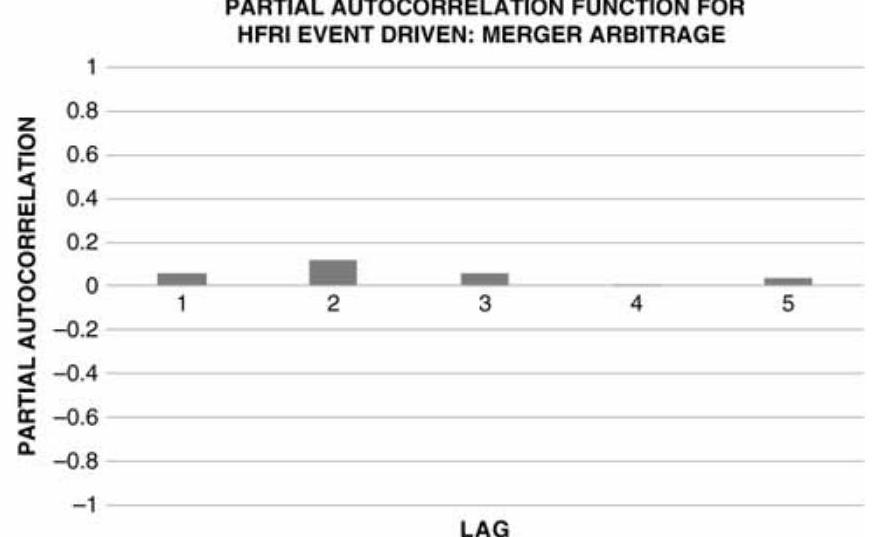
\includegraphics[max width=\textwidth]{2024_04_09_da1ba80afb4795888518g-5(1)}
\end{center}

Histogram of HFRI Event Driven: Merger Arbitrage Returns (Monthly) Jan. 2000-Dec. 2021

\begin{center}
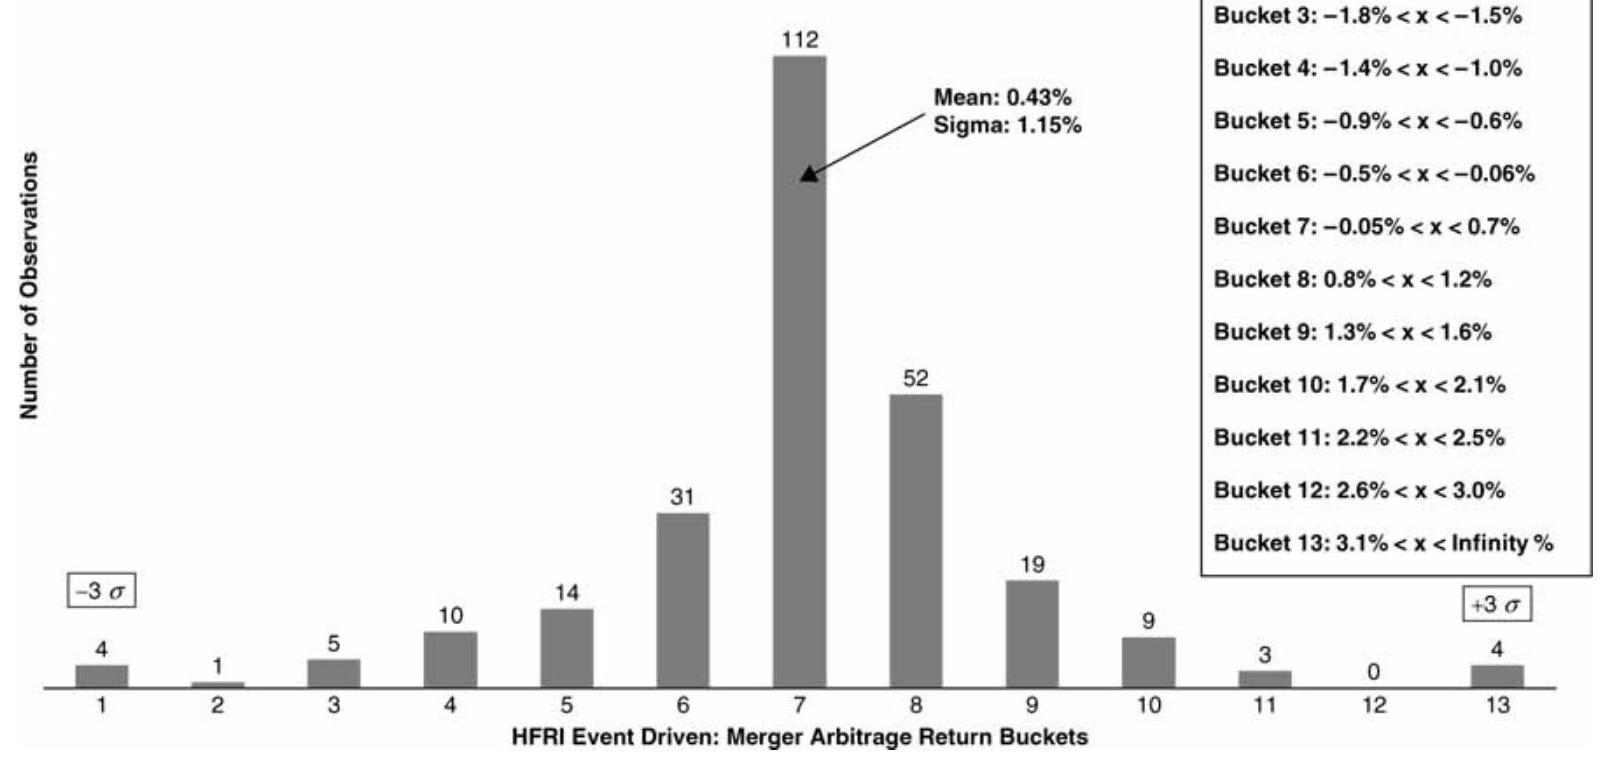
\includegraphics[max width=\textwidth]{2024_04_09_da1ba80afb4795888518g-5}
\end{center}

\section*{Statistical Summary of Returns}
Key observations on the returns to merger arbitrage funds that are consistent with economic reasoning are an essential component of knowledge and include the following:

\begin{enumerate}
  \item Merger arbitrage returns exhibited much lower volatility than world equities.

  \item Merger arbitrage returns exhibited lower skew and higher kurtosis than world equities.

  \item Merger arbitrage returns had a very favorable maximum drawdown.

  \item Merger arbitrage returns exhibited moderate positive autocorrelation, similar to world equities.

\end{enumerate}

\end{document}